\begin{problem}{Breytunafn}{Inn}{Út}{~}{~}

	\begin{wrapfigure}{r}{0.35\textwidth}
		\vspace{-25pt}
		\begin{center}
			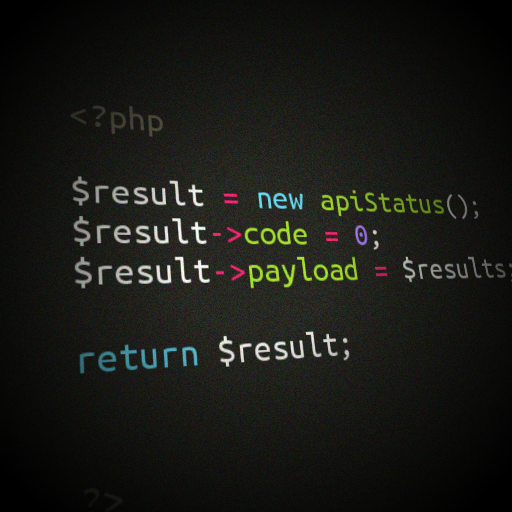
\includegraphics[scale=0.30]{../Breytunafn/code.png}
		\end{center}
		\vspace{-30pt}
	\end{wrapfigure}

	Flest forritunarmál leyfa forritaranum að vinna með svokallaðar breytur. Forritarinn getur sett gildi breytunnar, og svo seinna lesið gildi breytunnar. Yfirleitt eru ákveðnar reglur varðandi nöfn á breytum. Í þessu dæmi skulum við nota eftirfarandi þrjár reglur:

	\begin{enumerate}
		\item Nafn breytu má ekki vera tómi strengurinn
		\item Nafn breytu má aðeins innihalda enska bókstafi ('\texttt{a}`-'\texttt{z}` og '\texttt{A}`-'\texttt{Z}`), tölustafi ('\texttt{0}`-'\texttt{9}`) og undirstrik ('\_{}`)
		\item Nafn breytu má ekki byrja á tölustaf
	\end{enumerate}

	Skrifið forrit sem les inn streng og athugar hvort að hann sé löglegt nafn á breytu eða ekki.

	\Input
		Á fyrstu línu er heiltalan $1 \leq T \leq 100$, sem táknar fjölda prófunartilvika sem fylgja. Hvert prófunartilvik samanstendur af einni línu sem inniheldur strenginn sem á að athuga.

	\Output
		Fyrir hvert prófunartilvik á að skrifa út eina línu sem inniheldur "`\texttt{Valid}"' ef strengurinn er löglegt breytunafn, en "`\texttt{Invalid}"' annars.

	\Examples

		\begin{example}
			\exmp{
6
hello
x
\_{}Test123
10x
width!height
Color Of Horse
			}{
Valid
Valid
Valid
Invalid
Invalid
Invalid
}%
		\end{example}

\end{problem}